\chapter*{Part II --- Leaving the Cave}
\addcontentsline{toc}{chapter}{Part II --- Leaving the Cave}

In Part I, we laid the bedrock. We stripped away the comforting illusion that computation is merely a linear list of instructions waiting to be obeyed, one after another, like items on a checklist. Instead, we revealed it as \textbf{transformation}---a living, breathing process of mutation unfolding in structured time. We learned that systems are not flat maps drawn on a single plane, but deep, recursive \textbf{WARP graphs}, layering entire worlds inside of worlds, structure within structure, graphs nested in the edges of other graphs. We discovered that change is not random improvisation or chaotic state mutation; it is governed by the strict, typed physics of \textbf{Double-Pushout (DPO)} rewriting, a rule system that constrains what motions are even legal in the first place.

We have the particles. We have the laws of motion. We know how things change.

And yet, for all that structure, something crucial remains missing.

We know \emph{exactly} how the machine moves---step by step, rule by rule---but we do not yet know what it \emph{feels like} to be inside that motion. The mechanics of DPO explain \emph{how} a state transitions to its successor, but they remain silent on a more profound question: \emph{why} do some changes feel inevitable, almost gravitational, while others feel impossible, as if the universe itself refuses to permit them?

The mechanical model does not explain why debugging a race condition feels like getting lost in a labyrinth with no map, or why optimizing a hot loop feels like discovering a shortcut through a mountain range. It does not explain why two system states can look completely different on inspection yet behave identically under every possible input---as if they were secretly the same place wearing different masks. It does not explain why your entire system could have evolved into a radically different configuration if a single network packet had arrived one millisecond sooner, or one millisecond later.

To answer these questions, we need more than a model of \emph{execution}. We need a model of \emph{possibility}. We need to see the shape of computation itself.

Part II is where we give that shape a name.

Here, we zoom out. We pull back the camera until individual rewrites---the discrete, atomic steps that felt so important in Part I---blur together into something continuous. We stop obsessing over the single path the code actually took and start perceiving the vast, invisible landscape of \emph{possible} rewrites that surrounded that path at every moment. This is not an abstract notion. It is a real structure, a place with distinct neighborhoods of stability where computations tend to settle, and steep gradients of change where small perturbations cascade into wildly different outcomes. It has surfaces you can walk on. It has curvature that bends paths toward attractors or repels them toward chaos. It has worldlines---the actual geometric trajectories carved by real computations as they navigate through this ether of possibility.

This is the geometry of thought.

This is where computation stops being a process you \emph{run} and becomes a terrain you \emph{navigate}.

\begin{figure}[h]
    \centering
    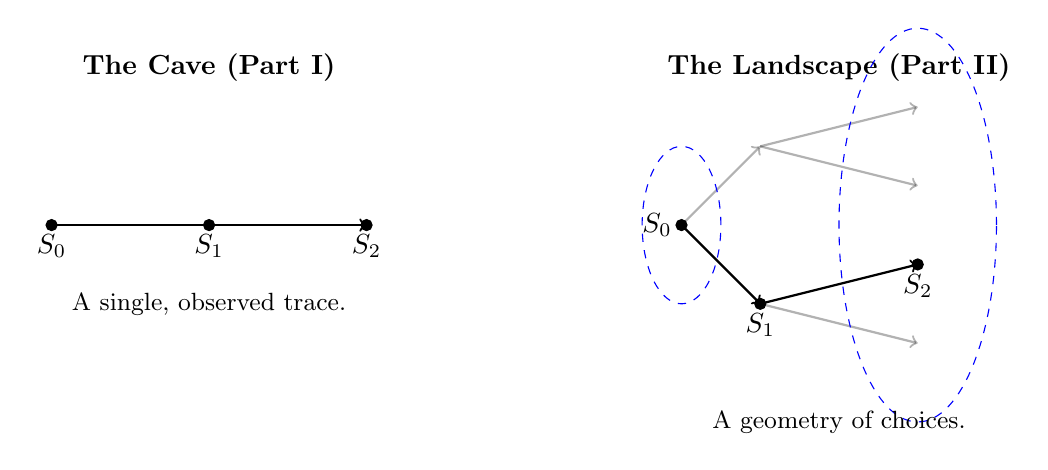
\begin{tikzpicture}
        % The "Cave" view: Linear path
        \node at (-4, 2) {\textbf{The Cave (Part I)}};
        \draw[->, thick] (-6,0) -- (-2,0);
        \filldraw (-6,0) circle (2pt) node[below] {$S_0$};
        \filldraw (-4,0) circle (2pt) node[below] {$S_1$};
        \filldraw (-2,0) circle (2pt) node[below] {$S_2$};
        \node at (-4, -1) {\small A single, observed trace.};

        % The "Landscape" view: Branching possibility
        \node at (4, 2) {\textbf{The Landscape (Part II)}};
        
        % Nodes
        \coordinate (O) at (2,0);
        \coordinate (A) at (3,1);
        \coordinate (B) at (3,-1);
        \coordinate (AA) at (5,1.5);
        \coordinate (AB) at (5,0.5);
        \coordinate (BA) at (5,-0.5);
        \coordinate (BB) at (5,-1.5);
        
        % Edges (The Worldlines)
        \draw[->, thick, opacity=0.3] (O) -- (A);
        \draw[->, thick] (O) -- (B); % Selected path
        \draw[->, thick, opacity=0.3] (A) -- (AA);
        \draw[->, thick, opacity=0.3] (A) -- (AB);
        \draw[->, thick] (B) -- (BA); % Selected path
        \draw[->, thick, opacity=0.3] (B) -- (BB);
        
        % The "Surface" visualization
        \draw[dashed, blue] (2,0) ellipse (0.5 and 1);
        \draw[dashed, blue] (5,0) ellipse (1 and 2.5);
        
        \filldraw (O) circle (2pt) node[left] {$S_0$};
        \filldraw (B) circle (2pt) node[below] {$S_1$};
        \filldraw (BA) circle (2pt) node[below] {$S_2$};
        
        \node at (4, -2.5) {\small A geometry of choices.};
    \end{tikzpicture}
    \caption{The shift in perspective: From a linear trace of what happened to the geometric manifold of what \emph{could} happen.}
    \label{fig:cave_vs_landscape}
\end{figure}

\section*{The Sky of Possibility}

Think of Part I as the Cave.

Inside the cave, your vision was limited to the mechanics. You learned to see the rules, the edges, the nodes, the deterministic ticks of the clock. You witnessed wormholes connecting distant regions of your graph, interfaces mediating between nested subworlds, and the raw machinery of motion grinding forward one DPO rewrite at a time. These are necessary foundations---you cannot understand the landscape without first understanding the ground beneath your feet. But they are ultimately just shadows on a wall. They are traces of what happened, footprints left behind, not the full reality of what \emph{is}.

In Part II, you step outside.

For the first time, you witness the \textbf{sky of possibility}.

You see not just what the system did, but the ghostly halo of what it \emph{could} have done. Every committed step, you now realize, casts a shadow of alternatives---paths not taken, rewrites that were legal but unchosen, entire histories that branched away into parallel trajectories the moment the scheduler made a decision. And here is the insight that changes everything: these alternatives are not random noise. They are not meaningless counterfactuals to be discarded. They have structure. They form a geometry of their own, a space with distance and direction and curvature. They are as real, in a formal sense, as the path you actually walked.

You begin to understand that the state of your system is not a point. It is a region in a much larger space---a neighborhood of near-identical configurations, surrounded by other neighborhoods, separated by gradients and barriers and basins of attraction.

You see \textbf{Aios} for what it truly is: not a mystical artifact or a philosophical abstraction, but the \emph{local shape of your computational freedom}. It is a finite, computable cone of possibility that opens outward from the vertex of \emph{now}, widening or narrowing as local constraints permit. The cone contains every legal move you could make from this moment forward. Its shape tells you how constrained or how free you are. Its boundaries tell you what the physics forbids. And the name is no accident: \textbf{AI$\Omega$N} derives from Aios. The framework is named for the geometry of possibility itself.

\begin{figure}[h]
    \centering
    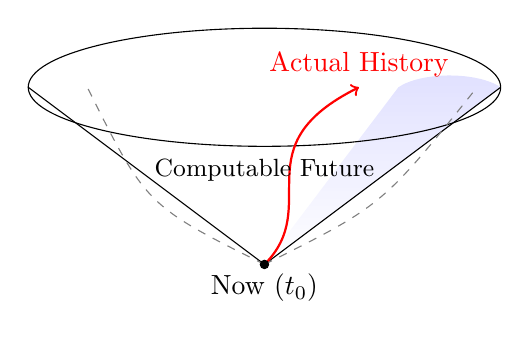
\begin{tikzpicture}[scale=1.5]
        % Base point
        \coordinate (Origin) at (0,0);
        
        % The Cone
        \shade[top color=blue!20, bottom color=white, opacity=0.6] 
            (0,0) -- (2,1.5) arc (30:150:0.5cm and 0.2cm) -- cycle;
        \draw (0,0) -- (2,1.5);
        \draw (0,0) -- (-2,1.5);
        \draw (0,1.5) ellipse (2cm and 0.5cm);
        
        % Worldline
        \draw[red, thick, ->] (0,0) .. controls (0.5, 0.5) and (-0.2, 1) .. (0.8, 1.5) node[above] {Actual History};
        
        % Alternative paths
        \draw[gray, dashed, thin] (0,0) .. controls (-1, 0.5) .. (-1.5, 1.5);
        \draw[gray, dashed, thin] (0,0) .. controls (1, 0.5) .. (1.8, 1.5);
        
        \filldraw (Origin) circle (1pt) node[below] {Now ($t_0$)};
        \node at (0, 0.8) {\small Computable Future};
    \end{tikzpicture}
    \caption{Aios: the local cone of valid DPO rewrites available from any given state. The red line is the path actually taken; the dashed lines are the ghosts of paths not chosen.}
\end{figure}

In this light, determinism reveals itself as simply a line drawn in the sand---the single trajectory you committed to---while choice reveals itself as geometry. The shape of what you \emph{could} do is as important as the history of what you \emph{did}. Optimization, then, is not about ``making the code faster.'' Optimization is navigation: finding shorter paths through this space. Debugging is not about ``finding the bug.'' Debugging is archaeology: tracing a worldline backward through the geometry until you locate the wrong turn.

\section*{What Part II Will Teach You}

Part II is about learning to walk this landscape with your eyes open.

Leaving the cave is not about enlightenment in some mystical sense. It is not about transcending the details or escaping into pure abstraction. Quite the opposite. It is about finally seeing the \textbf{full dimensionality} of the system you have been working inside all along. The single execution trace you observed in Part I was always embedded in a much larger structure. You just could not see the embedding. Now you will.

In the chapters ahead, we will formalize this intuition. We will define Rulial Space---the manifold of all possible computations under a given rule system. We will define Rulial Distance---a way to measure how ``far apart'' two computational states really are, not in terms of superficial differences, but in terms of the rewrites required to transform one into the other. We will trace worldlines through this space and discover that they obey geometric laws, bending toward attractors and avoiding forbidden regions.

By the end of Part II, you will have a new vocabulary for the questions that have always haunted systems engineering. You will understand why some bugs feel ``close'' and others feel ``unreachable.'' You will understand why certain optimizations are cheap and others are expensive in a way that has nothing to do with CPU cycles. You will understand why two programs that look nothing alike can be, in a deep geometric sense, the same program.

You do not escape into abstraction here. You step into clarity.